\documentclass[12pt]{article}
\usepackage[paperheight=11.5in,paperwidth=8.65in,margin=0in]{geometry}

% postscript courier and times in place of cm fonts
\usepackage{courier}
\usepackage{times}

\usepackage{graphicx}
\usepackage[dvipsnames]{xcolor}
\usepackage[prologue,table]{pstricks}
%\usepackage{pst-grad}
%\usepackage{pst-ghsb}
%\usepackage{pst-slpe}

% define colors
%\definecolor{CodeBackGround}{cmyk}{0.0,0.0,0,0.05}     % light gray
%\definecolor{CodeComment}{cmyk}{0.0,0.0,0,0.07}        % light gray
%\definecolor{CodeComment}{rgb}{1,0.5,0}                % orange {1,0.5,0} 
%\definecolor{CodeComment}{rgb}{0,0.08,0.45}            % dark blue {0,0.08,0.45}
\definecolor{CoverColor}{rgb}{0,0.80,0.08}             % dark green {0,0.45,0.08}
\definecolor{TitleColor}{rgb}{0,0.35,0.08}             % pure white{1,1.00,1.00}
\definecolor{BackTextColor}{rgb}{0,0.35,0.08}          % 

\begin{document}
\thispagestyle{empty}

\newsavebox\IBackBox
%\sbox\IBackBox{\includegraphics[height=11.5in]{jod_clouds.eps}}
\sbox\IBackBox{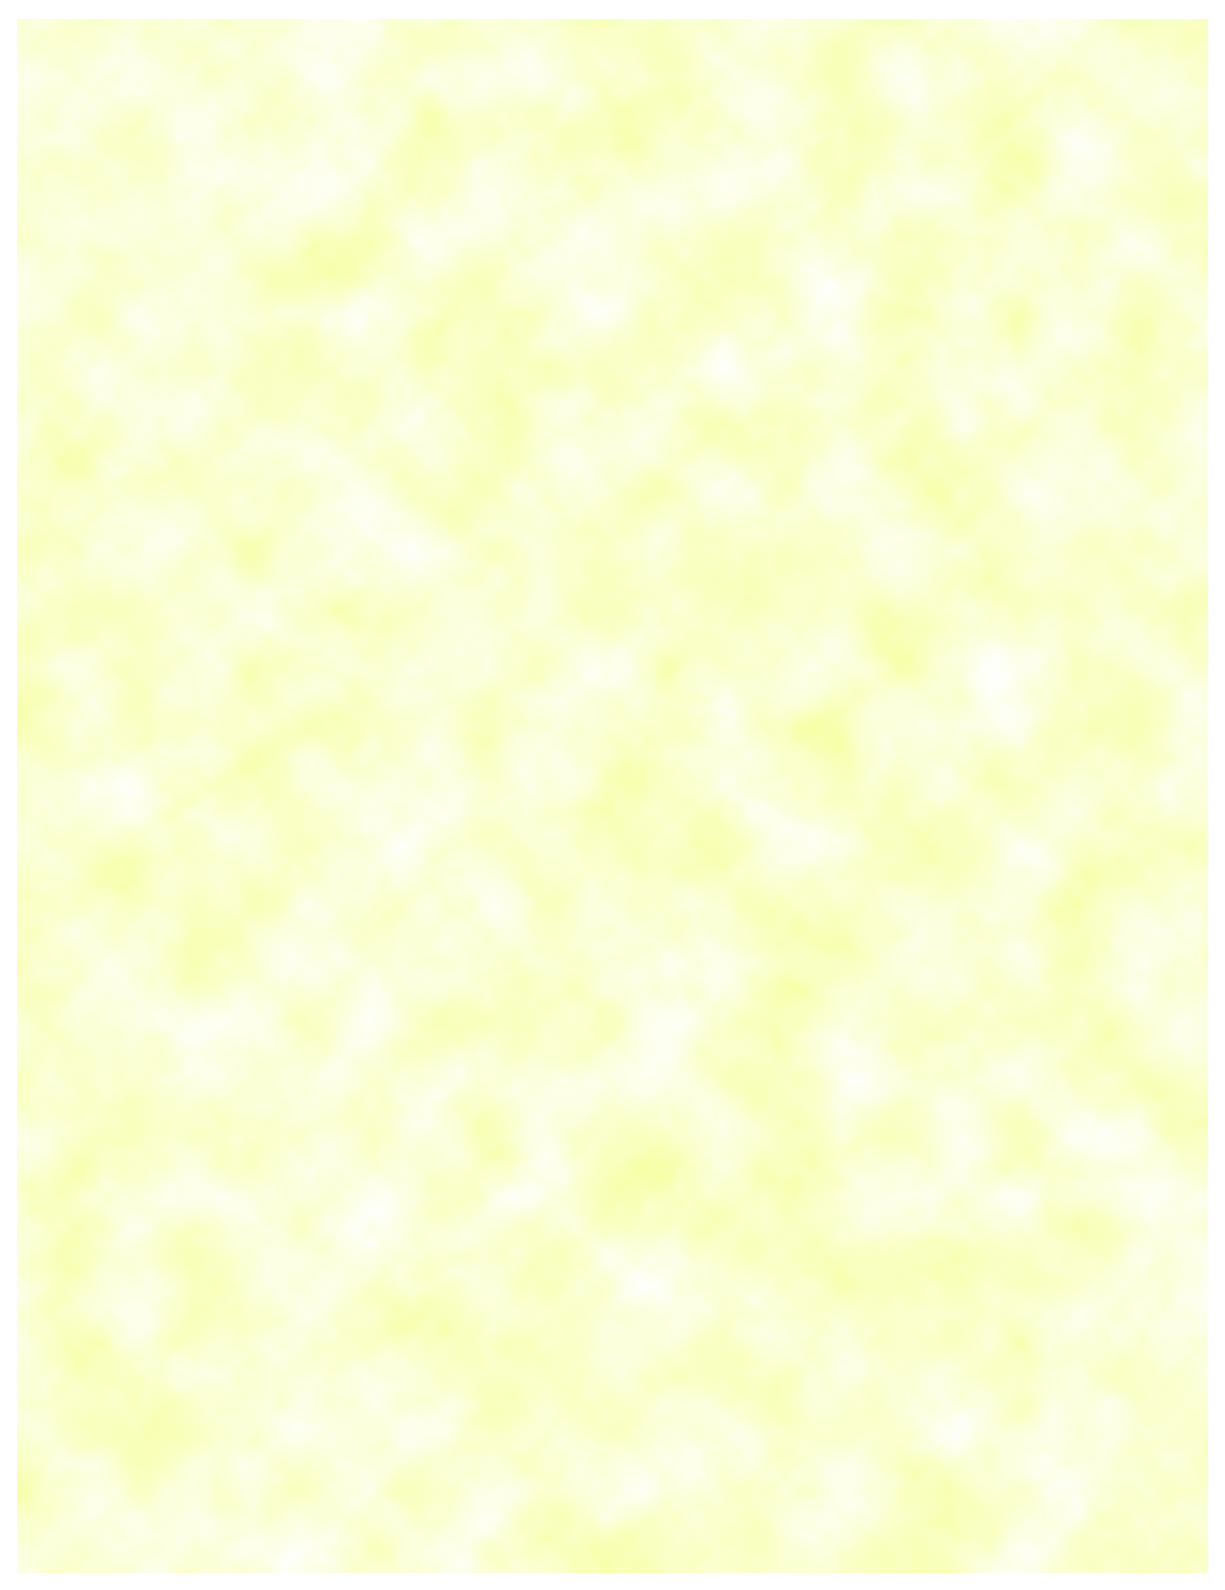
\includegraphics[height=11.5in]{jod_85x11_back_2.eps}}

\newsavebox\IAuthorBox
\sbox\IAuthorBox{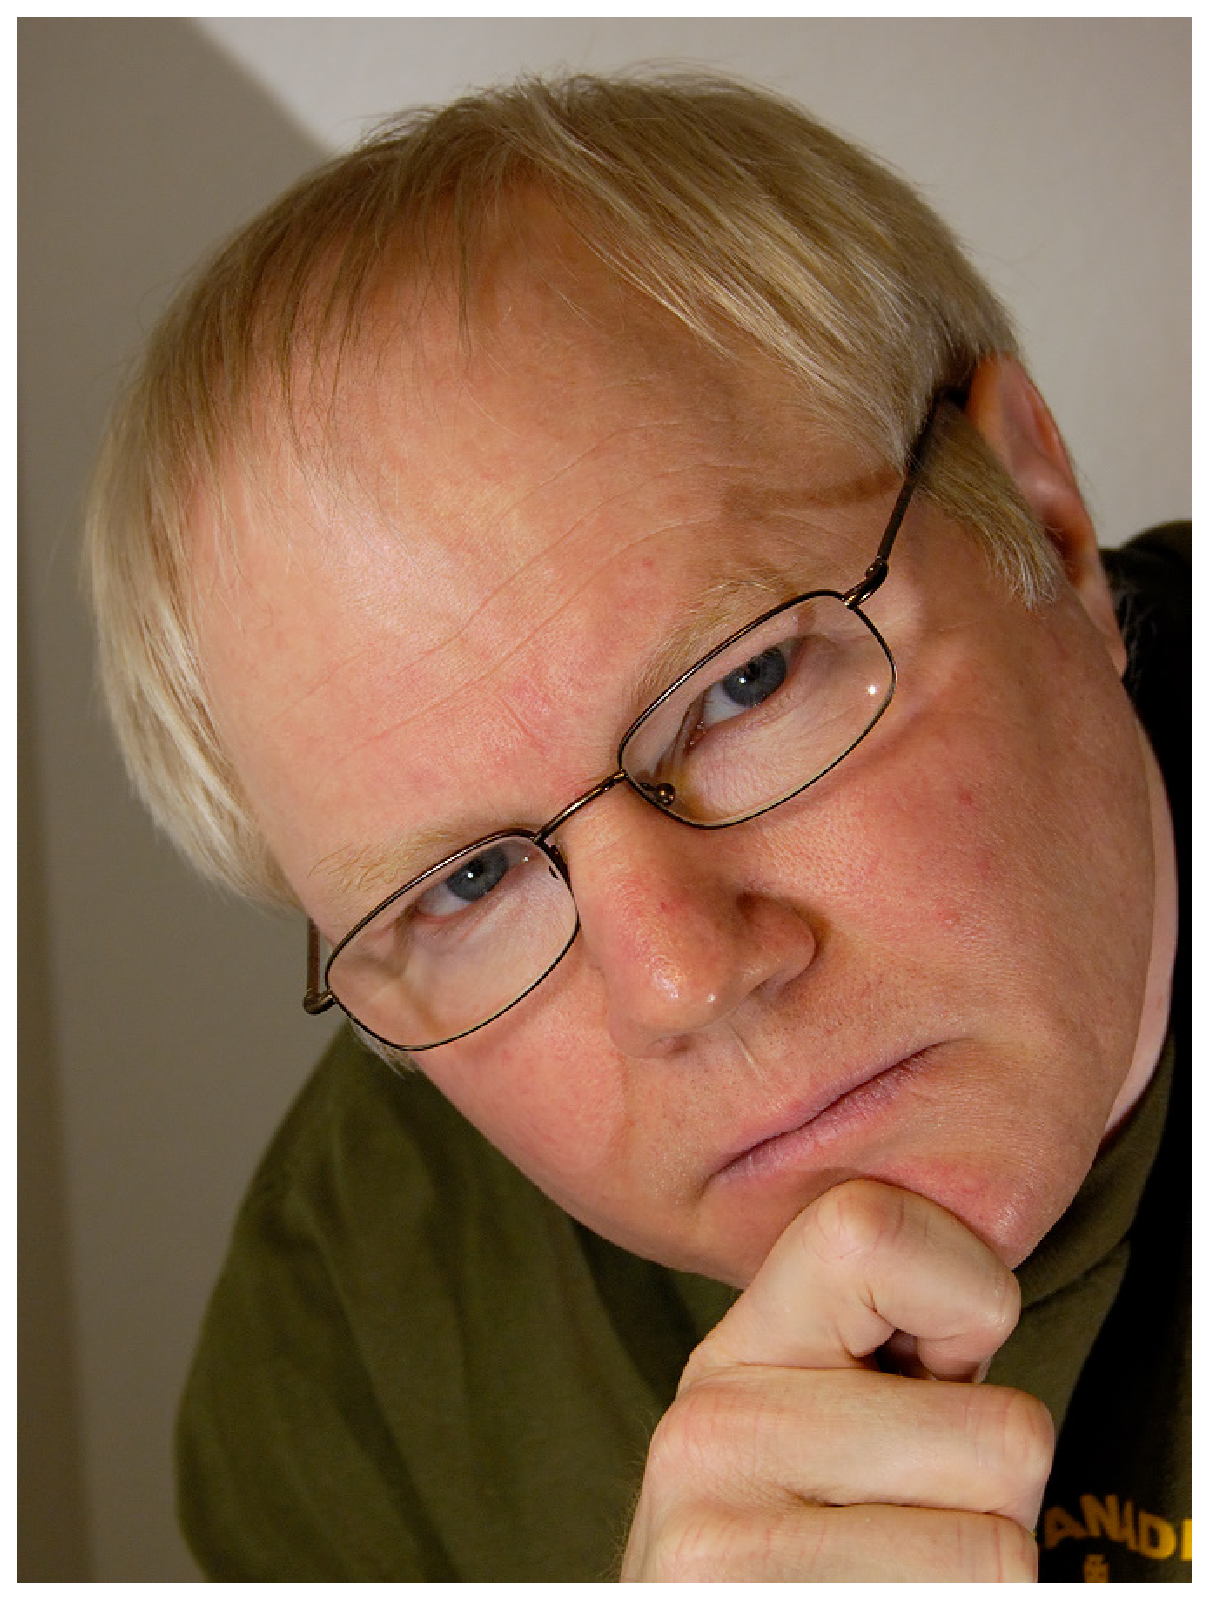
\includegraphics[height=3.2in]{author.eps}}

\newsavebox\BioBox
\sbox\BioBox{\begin{minipage}{4.0in}

\textcolor{BackTextColor}{In 1991 I read a \texttt{USENET} message about a new 
Kenneth Iverson designed programming language called J.  APL, Iverson's 
first programming language, had deeply influenced me so I knew J was 
worth a look. J did not disappoint. J's rare combination of theoretical 
coherence, productivity, array orientation and elegance is a daily delight.}

\medskip

\textcolor{BackTextColor}{JOD is a J programming tool that reflects my 
word oriented approach  to J coding. The inspiration for JOD comes 
from Roger Hui and Kenneth Iverson's \emph{Dictionary of J}: a seminal 
document that correctly highlights the power of the J word.} 


\begin{flushleft}
\textcolor{BackTextColor}{John D. Baker}

\textcolor{BackTextColor}{December 2011}

\textcolor{BackTextColor}{St. Louis, Missouri}
\end{flushleft}

\end{minipage}}

\DeclareFixedFont{\PT}{T1}{ppl}{b}{n}{0.78in}
\DeclareFixedFont{\PTsmall}{T1}{ppl}{b}{it}{0.4in}
%\DeclareFixedFont{\PTsmallest}{T1}{ppl}{b}{it}{0.3in}
%\DeclareFixedFont{\PTtext}{T1}{ppl}{b}{it}{11pt}
%\DeclareFixedFont{\Logo}{T1}{pbk}{m}{n}{0.3in}


\psset{unit=1in}
\begin{pspicture}(8.625in,11.25in)
\psframe[fillstyle=solid,fillcolor=CoverColor](-0.40,0.0)(8.65,11.5)

% background image
\rput[lb](-0.40,0.0){\usebox\IBackBox}

% bio text box
\rput[tl](3.3,9.4){\usebox\BioBox}

% author image
\rput[lb](0.65,6.25){\usebox\IAuthorBox}


\end{pspicture}

\end{document}